\section{Real-World Configuration Changes}
\label{sec:study}

In the software engineering literature, despite a rich body of
software change analysis work~\cite{STVR:STVR1475, Dagenais:2008, Tao:2012:SEU}, 
software configuration changes across multiple
versions are less studied. Do configuration
changes arise during software evolution in practice?
This section describes an initial study of
\studysubjnum  real-world configurable systems to answer
this question.
% to investigate whether
%and how configuration changes arise during software evolution.
%\todo{say the object is whether such changes
%often exist in practice?}
%\todo{perphas the study purpose should be toned down a bit. donot
%claim too much. just say whether configuration changes are frequent or not.}

%Knowing whether and how configuration options evolve in practice
%can be beneficial for both software developers
%and tool designers. For example, knowing what types
%of configuration changes are common in practice
%can help developers improve the current designs and
%implementations to create better systems or documentations
%; for tool builders, so that they can improve their tools
%to match reality (e.g., by knowing the types of configuration
%changes that occur most frequently).


\begin{table}[t]
\vspace{1mm}
\centering
\small{
\setlength{\tabcolsep}{.40\tabcolsep}
\begin{tabular}{|l||c|c|c|c|}
\hline
 Program & Versions & Years & LOC (latest version)  & Language\\
 \hline
 \hline
 MySQL & 5.1, 5.5, 5.6, 5.7 & 3 &1565212& C/C++\\
 Apache& 2.0, 2.2, 2.4 & 3  & 139178 &C/C++\\
 Firefox& 7.0--22.0 (16 versions) & 3  & 8237915&C/C++\\
 Randoop & 1.2.1, 1.3.2, 1.3.3 & 6 & 19511   &Java\\
 Weka & 3.4, 3.5, 3.6, 3.7  & 2  & 288369 &Java\\
 JChord & 1.0, 2.0, 2.1 &  4 & 26617  &Java\\
 Synoptic & 0.04, 0.05, 0.1 & 2   & 19153 &Java\\
 JMeter & 2.6, 2.7, 2.8, 2.9& 2   & 91979 &Java\\
\hline
\end{tabular}
}
\vspace{-2mm}
\Caption{{\label{tab:subjects} The open-source
software systems we studied and their characteristics.
Column ``Years'' is the active development period
for the selected versions. 
}
}
\end{table}


\begin{table}[t]
\vspace{1mm}
\centering
\small{
\setlength{\tabcolsep}{.50\tabcolsep}
\begin{tabular}{|l||c|c|c|c|}
\hline
 Program & \#Added Options & \#Deleted Options& \#Modified Options\\
 %&  Options &  Options&  Options \\
 \hline
 \hline
 MySQL& 26 & 24 & 23 \\
 Apache & 5 & 0 & 10 \\
 Firefox& 28 & 7 & 56 \\
 Randoop & 37  & 26 & 2\\
 Weka &  72 & 4 & 13 \\
 JChord & 13  & 10 & 5 \\
 Synoptic & 3 & 0 & 2 \\
 JMeter & 17  & 3 &  12 \\
\hline
\hline
 Total & 201 & 70 & 123 \\
\hline
\end{tabular}
}
\vspace{-2mm}
\Caption{{\label{tab:options} The total number of new, deleted,
and modified configuration options for each subject program
in the studied versions.
%\todo{Are the added options interesting from the point of view of this
%  paper?  They never contribute to configuration errors, do they?  If so,
%  explain.  If not, remove them from all the tables.}
}
}
\end{table}


\begin{table}[t]
\vspace{1mm}
\centering
\small{
\setlength{\tabcolsep}{.50\tabcolsep}
\begin{tabular}{|c|c|}
\hline
 \textbf{Change Type} & \textbf{Description} \\
 \hline
 \hline
Bugs & Fix existing bugs\\
 \hline
Renaming & Change the option name\\
 \hline
Features & Add, remove, or modify features\\
 \hline
Reliability & Improve reliability or performance\\
 %\hline
%Maintainance & Maintain the code and documentation \\
%& (e.g., renaming the option name) \\
\hline
\end{tabular}
}
\vspace{-2mm}
\Caption{{\label{tab:conftypes} Types
of configuration changes identified in our
study from the subject programs in Table~\ref{tab:subjects}.}
}
\end{table}

\begin{table}[t]
\vspace{1mm}
\centering
\small{
\setlength{\tabcolsep}{.50\tabcolsep}
\begin{tabular}{|l|c|c|c|c|}
\hline
 Program & \multicolumn{4}{|c|}{\textbf{\#Changed Configuration Options}} \\
 \cline{2-5}
 & Bugs & Renaming & Features & Reliability \\
 \hline
 \hline
 MySQL & 0 & 15 & 55 & 3 \\
 Apache& 0 & 0 & 11 & 4 \\
 Firefox& 28 & 0 & 55 & 8 \\
 %FindBugs & & & & \\
 Randoop & 0  & 2 & 62  & 1\\
 Weka & 1  & 0 & 81  & 8 \\
 JChord & 0  & 2 & 24 & 2\\ %add a default file
 Synoptic & 0 &  5 & 0 & 0\\
 JMeter & 7  & 0 & 18 & 7 \\
\hline
\hline
 Total & 36 & 24 & 301 & 33 \\
\hline
\end{tabular}
}
\vspace{-2mm}
\Caption{{\label{tab:categories} The number of configuration changes of
each type (Table~\ref{tab:conftypes}).}}
\end{table}


\subsection{Subject Programs and Study Methodology}


Table~\ref{tab:subjects} lists
\studysubjnum open-source configurable systems used in our
study.
% The \studysubjnum subjects contains
% three C/C++ software systems and six Java software systems.
MySQL~\cite{mysql}  is a popular relational database management
system. Apache~\cite{apache} has been a dominant
HTTP server on the Internet since 1996. Firefox~\cite{firefox}
is an open-source browser available on multiple platforms.
Randoop~\cite{randoop} is an automated test generator for Java
programs. Weka~\cite{weka} is a toolkit that implements machine
learning algorithms. JChord~\cite{jchord} is a program analysis platform that
enables users to design and implement static and
dynamic program analyses for Java. Synoptic~\cite{synoptic} mines a
finite state machine model representation of a system from
logs. JMeter~\cite{jmeter} is a tool to load test functional
behavior and measure performance.
Each program is highly configurable, and has evolved over
a considerable amount of time for the selected versions ({2--6} years).


In our study, %rather than searching bug repositories,
we manually examined the revision history of each subject program,
and searched for a set of 5 keywords (``configuration option'',
``add option'', ``delete option'', ``rename option'', and ``change option'')
in commit messages as well as in the change logs.
We searched 7022 commit messages and 28 change log entries, in
which 422 commit messages and 28 change log entries were matched.
For each match, we read the description of the change,
and the ``diff'' of the original file to check whether
the change is made to a configuration option. We collected
394 distinct configuration changes in total.
%and the
%changed file. This information indicated
%to us whether the change is related to how the
%software should be configured.

%We identifies the
%changed code and its affected configuration options
%manually.



\subsection{Findings}

Table~\ref{tab:options} summarizes the identified
configuration changes for each subject program.
Table~\ref{tab:categories} further classifies the
configuration changes into four categories shown
in Table~\ref{tab:conftypes} (each change belongs to a single category).


As shown in Table~\ref{tab:options}, configuration changes occur
in the evolution of every subject program. In fact, they occur in
every revision of each subject program (not shown in Table~\ref{tab:options},
due to space limits).  
%During software evolution, 
%developers frequently add \todo{xx}

As shown in Table~\ref{tab:categories},
feature-related configuration changes are the largest group across
all subject programs. These changes include
adding new configuration options to customize a program's
functionality, deleting existing options, or modifying the default
value of an option. 

Configuration evolution can have unexpected impact on
program behavior. After configuration changes, reusing
the existing configuration for an old software version
may yield a misconfiguration, causing different results
on the new version.  As described in Section~\ref{sec:evaluation},
our evaluation focused on deleted and modified options.
Adding new configuration options is less likely to cause
a configuration error.
%, since most of the added options are
%used in new software features, which are not available in
%the old version. Some newly added options are introduced
%to modify existing features, but they are disabled by
%default and will not have any effects on the new program
%version unless been explicitly turned on. For the deleted
%and modified options, they are more likely to affect a
%program's existing behavior. In our evaluation (Section~\ref{sec:evaluation}),
%we focused on deleted and modified options, and reproduced \errornum
%user-visible misconfigurations caused by them
%in the 5 Java programs of Table~\ref{tab:options},
%by following the change description and user manual.


%Regarding the impact of configuration changes, 

% \todo{I would cut this entire paragraph.  I don't see it as contributing much.}
% \todo{need a transition sentence here. do not claim much
% for this initial study.}
% Many of such configuration changes listed in Table~\ref{tab:options},
% perhaps except for changes to fix a reported bug\todo{but that changes
%   behavior, too, doesn't it?}, can affect
% a software's behavior. As described in Section~\ref{sec:evaluation},
% we produced XXX configuration errors for all 5 Java programs.
% Such XXX configuration errors include both crashing and non-crashing errors.


%\todo{normal examples}
%The following are options obsolete and have been removed in
%MySQL 5.5. Where alternatives are shown, applications should
%be updated to use them
%\todo{need rephrase}

%\todo{example}


%\vspace{1mm}
%\noindent\textbf{Examples}



\begin{figure*}[t]
  \centerline{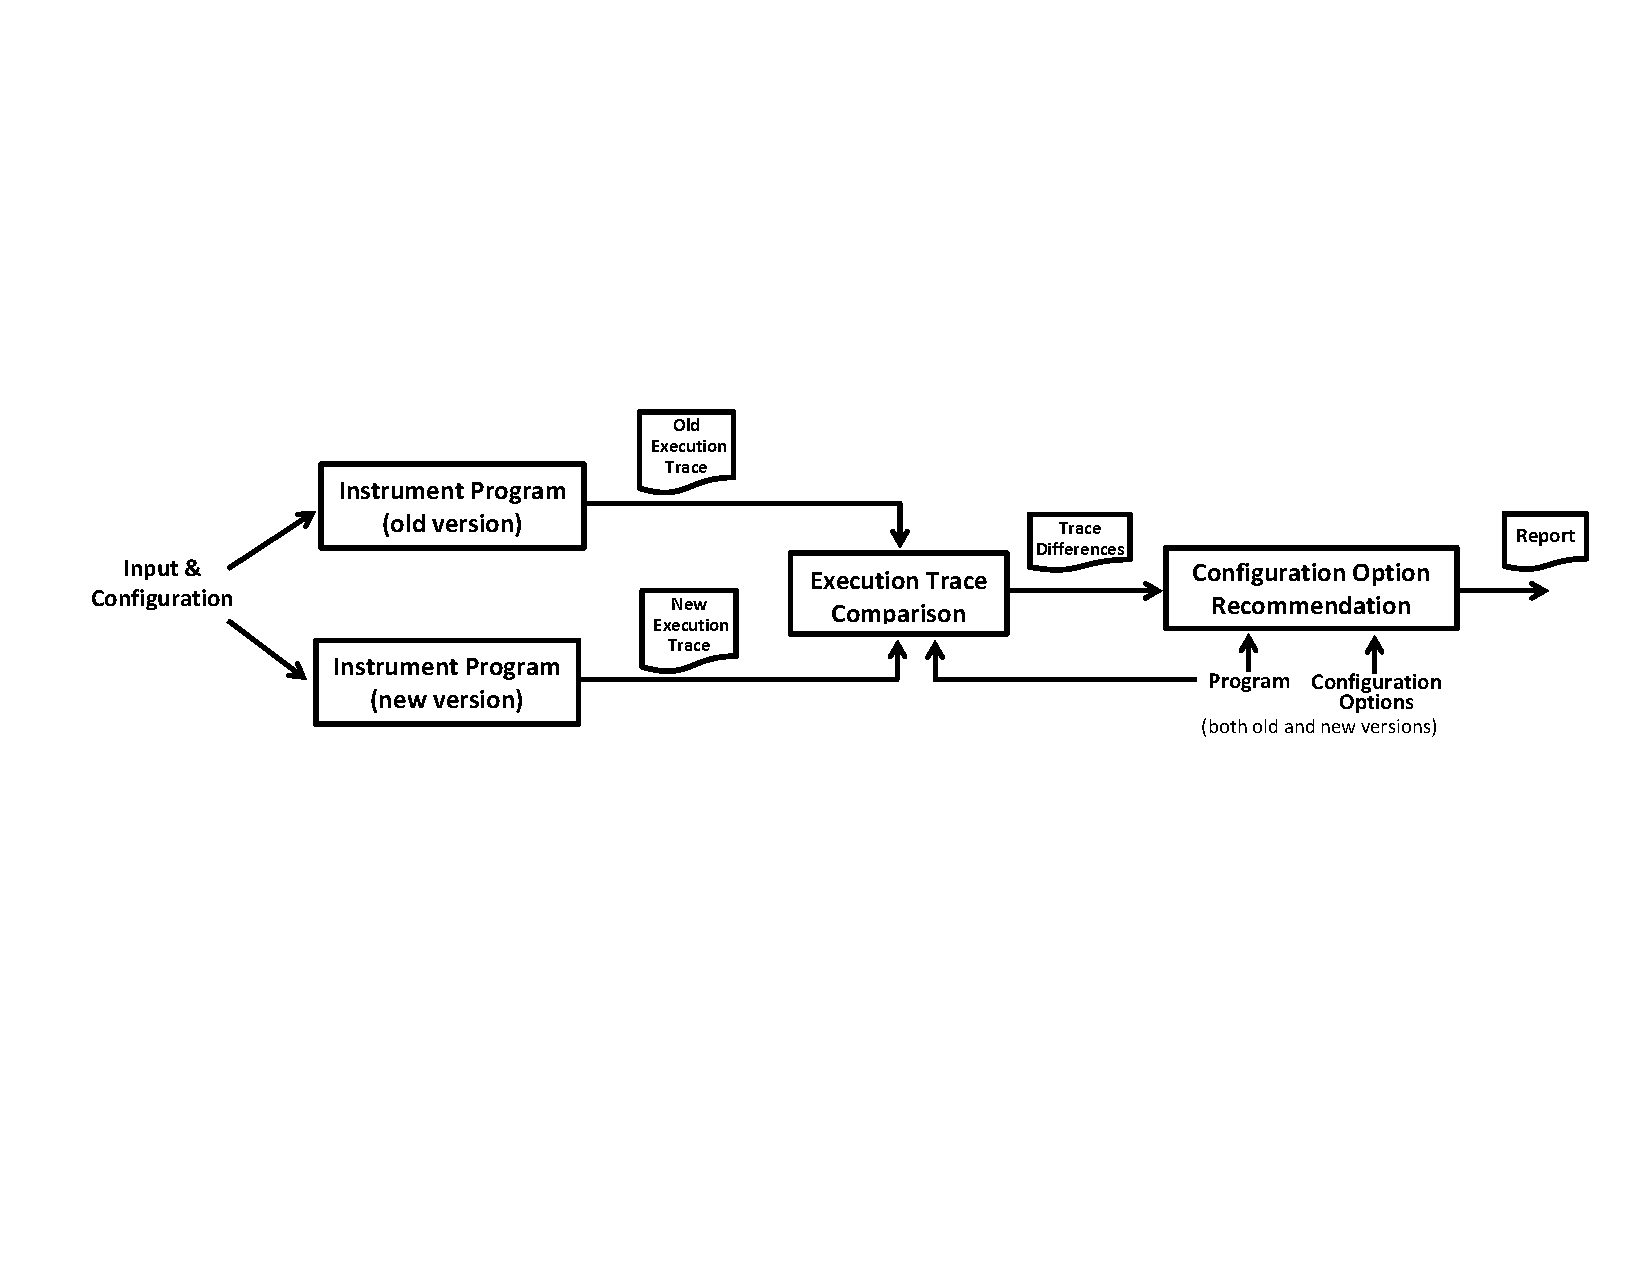
\includegraphics[scale=0.69]{workflow}}
  \vspace*{-2ex}\caption {{\label{fig:overview} The architecture of
  our \ourtool technique. The instrumented program versions and
  two execution traces are produced by the step in
  Section~\ref{sec:profiling}. 
  The ``Execution Trace Comparison'' step is described in
  Section~\ref{sec:comparison}. The ``Configuration Option Recommendation'' step
  is described in Section~\ref{sec:rootcause}.
}}
\end{figure*}


%\subsection{Summary}
%\subsubsection{Implications}

%Our study has three chief findings:
%\textbf{(1)} configuration
%changes arise frequently during software evolution: for
%all subject programs we have studied, every version
%includes configuration changes. \textbf{(2)} most configuration
%changes fall into a small number of types, among
%which \todo{most of them are feature related.}
%and \textbf{(3)} a large number of
%configuration changes may affect a program's
%behaviors. Users must properly reconfigure a
%program in order to maintain its original behavior.
%\todo{rephrase above. the purpose is to
%illustrate configuration change is prevalent}

%Our study also indicates that configuration errors
%can be frequent... \todo{xxx}
%\textbf{Implications.} If a user ignore the changes, even if the tests
%all pass. User-driven

\subsection{Threats to Validity}

Our findings apply in the context of our subject programs and methodology;
they may not apply to arbitrary programs.

The configuration changes identified by our methodology are
certainly not complete. Our keyword search might have missed some configuration changes.
Our methodology only studies changes that are directly made to a
software configuration option. We may miss
code or environment changes that indirectly affect the software behavior
and require users to re-configure the new software version.

%We only examined software change logs to identify changed configurations, which is a biased
%subset; there may be (many) other configuration
%options are affected by code changes. 

%A similar study that leverages the recent advance in
%change impact analysis~\cite{} may be needed
%to identify a more complete set of configuration changes.


%Our study is limited by the open-source
%software systems we chose, which may not reflect
%the characteristics of other software systems.
